\chapter{Result and evaluation}

\section{Result}

% Với mục đích xóa bỏ rào cản cho người khiếm thanh, khiếm thính. Nhóm đã tạo ra một ứng dụng sử dụng trí tuệ nhân tạo để nhận diện các cử chỉ thao tác thủ ngữ, từ đó có thể thông dịch trực tiếp ra tiếng Việt.
To remove barriers for people who are deaf or hard of hearing. The team developed an artificial intelligence application that recognizes gestures, manipulates words, and directly translates them into Vietnamese.

% Demo cho hệ thống được trình bày tại đây: ....

To watch the application's demo video, scan the QR code below or copy this url to your browser: \url{https://www.youtube.com/watch?v=Gn8mdojQnqY}

\begin{figure}[H]
	\centering
	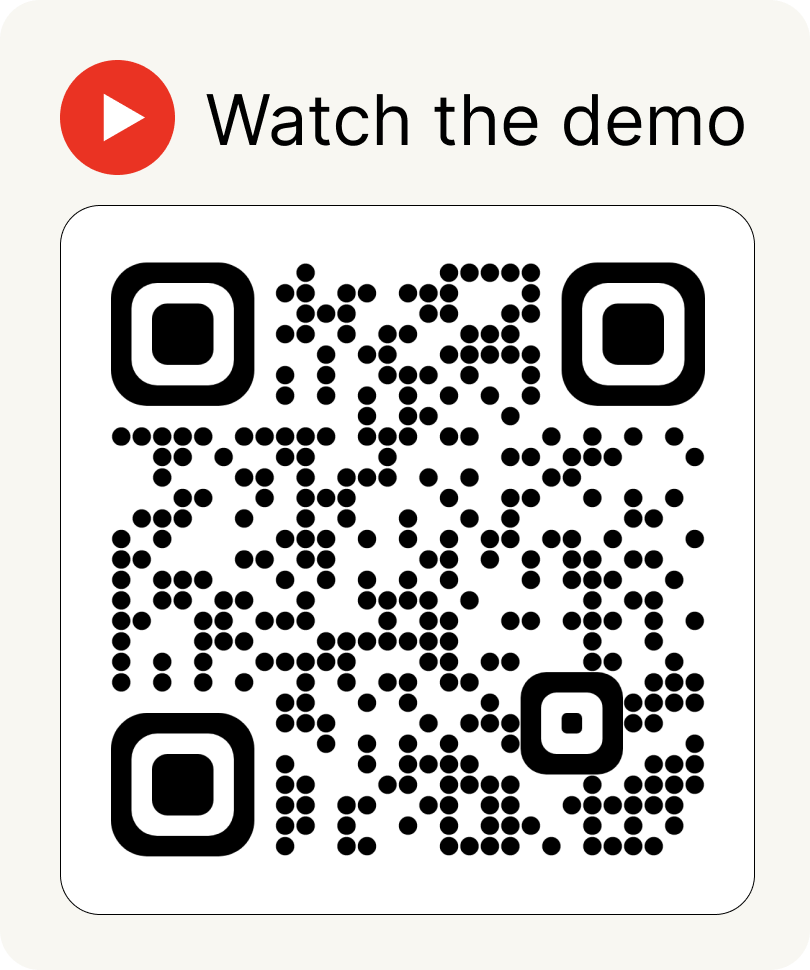
\includegraphics[width=0.5\textwidth]{img/qrcode_to_demo.png}
	\caption{The QR Code of the demo video}
  \label{fig:qrcode_to_demo}
\end{figure}

% Bên cạnh đó, với các kết quả đạt được, nhóm cũng đã thực hiện các thủ tục để có thể xin cấp quyền sở hữu trí tuệ cho sản phẩm và đang được chờ xét duyệt.

Moreover, with the results obtained, the group has completed procedures to apply for intellectual property rights for the product and is awaiting approval.

% Tuy nhiên, hệ thống vẫn có những nhược điểm nhất định như: với các thủ ngữ dài, phức tạp và cần nhiều thao tác thì hệ thống đề xuất không thể nhận diện được. Thời gian để hệ thống nhận diện một thủ ngữ tùy vào mức độ phức tạp vẫn còn chậm.

Nevertheless, the system still has some drawbacks, such as long, complex terms and a large number of operations that the proposed system cannot recognize. The system still takes a long time to recognize a sign language, depending on its complexity.

\section{Evaluation}
% Từ những kết quả đã hiện thực được, nhóm cũng có những kế hoạch, định hướng để hệ thống trở nên hoàn thiện hơn như sau:

Based on the actual results, the group has the following plans and orientations to make the system more complete:

\begin{itemize}
  \item Convert the application to use react-native in the end to meet the needs of both the Android and IOS platforms.
  \item Improve the system and correct any errors.
\end{itemize}










